\section{Design} \label{sec:design2}
This chapter introduces key concepts to enhance the understanding and technological framework of the Internet of Value (IoV). We propose a new architectural approach to increase efficiency in asset sharing within blockchain ecosystems using agentic systems. This approach is in accor-
dance to my dissertation targets discussed in Chapter \ref{sec:aims}.
We are primarily focusing Polkadot and the Substrate-based chains, with additional support of RISC-V-based Ethereum Virtual Machine (EVM) These concepts can also be adapted for other blockchain architectures like Solana. However, it is imporant to mention that as  Internet of Value is a very broad concept, our domain knowledge would be oriented around AI agent, value creation and sharing.

\subsection{Internet of Value in agentic system}

Paraphrasing Lohmer et al. \cite{Lohmer2024}, Internet of Value (IoV) can be defined as follows:
The internet of value enables the direct transfer of assets of any kind as well as processing and settlement of business transactions based on blockchain technology in conjunction with digital platforms, tokens, smart contracts, and other technologies such as the internet of things and artificial intelligence.
Its principles are to create a system compliant with data protection values, equal and fair access for all participants, effective representation of digital and physical assets, and disintermediation for direct peer-to-peer communication and the exchange of values
These technologies and principles facilitate open content and value sharing, transparency, sustainable behavior, and self-sovereign digital identities.
IoV creates an ecosystem where platforms enable value exchange across various types of digital and physical assets. Blockchain technology ensures that these exchanges are secure, transparent, and decentralized.

This definition emphasizes the role of blockchain technology as the foundational enabler, working in conjunction with other technologies like digital platforms, tokenization, smart contracts, Internet of Things, and artificial inteligence. As the main goal of the IoV is the ability to transfer and process various types of assets and transactions directly, where every participant has equal access to the assets. Assets should be effectively represented without any need of trusted-third party. Therefore outcome of platforms in the IoV should be transparent, sustainable, and self-sovereign.

What are plaforms?  Platforms are digital infrastructures that act as intermediaries between different actors. This is a broad definition, but it is important to understand that platforms are not just websites or apps. Platforms can be physical or digital, and they can be used to facilitate the exchange of goods, services, or information. As internet became more accessible to the people\footnote{That smatphones became usable (iPhone 3G)}, gig economy has emerged. Gig economy is a labor market characterized by the prevalence of short-term contracts or freelance work as opposed to permanent jobs. This is a good example of how platforms can be used to create new markets, disrupt existing markets, or enable new forms of collaboration. Platforms therefore create a new socio-economic model in which people offer under-utilized access with temporary access to others. Therefore we can sat that the objective of plaforms in the sharing economy is to provide under-utilized asset to gain profit.
In short: to exchange value. How are these platforms able to create value? In the context of blockchain we need a way to digitize assets into the blockchain. This is where tokenization comes into play. Tokenization is the process of digitally representing uniquely identifiable assets, with proof of ownership registered using blockchain technology. Using smart contracts and few notable token standards, assets can be tokenized and exchanged in a secure and transparent way. In practise, assets based on their fungibility are tokenized based on ERC-20, ERC-721, ERC-1155, or other standards. What makes blockchain-based platforms unique in opposed to centralized solution is that based on the token stnadards, we are able to leverage the composability of the tokenzied assets. If we take traditional platforms based on centralized solution, we would have hard time to implement all the possible APIs into one roof. However, thanks to the token standards we do not have huge deviations between the tokenized assets. Therefore buiding platforms that levarage tokens is much easier.

In summary Internet of Value is network which provides a space for platforms that can create and share value for network participants.
How do agentic systems fit into Internet of Value? As we can observe, the primary unit of the Internet of Value is the asset.
The asset can be anything from a car to a house to a digital token, on the othe hand the in the Internet of Agents the primary unit is the Autonomous agents or in short LLM‑backed processes.
The cooperation of these two world lies in the fact that IoV solves the problem of trust and transparency in transactions, while agentic systems provide the intelligence and automation needed to facilitate these transactions.
To be more precise IoV solves the settlement where as agentic systems solve the cognition and processing.
By combining these two concepts, we can create a more efficient and effective system for sharing and exchanging value.

However, in general value is a concept that is difficult to define in a general sense, as it is subjective and context-dependent. As we mentioned in the Chapter \ref{sec:aims}, Lohmer et al. \cite{Lohmer2024} developed a comprehensive definition and framework of IoV through expert interviews. From their research they concluded a multi-dimensional notion of value where they encompass  Economic worth, Utility or access rights and Ethical and sustainability contributions. Based on these propositions we have defined value as a function of availability, durability and utility.

\begin{equation}
  Value = f(Availability, Durability, Utility)
\end{equation}

Why have we decided for this definiton? That is a valid question. To distill this into a clear idea we need to agree on the definitions of availability, durability and utility in the context of our work. Availability represents the asset’s scarcity, durability measures its longevity, and utility captures its functional benefits. Each of these components plays a role in determining the overall worth of an asset."

Therefore the three main components of value are:
\begin{itemize}
    \item \textbf{Availability:} The scarcity or abundance of an asset.
    \item \textbf{Durability:} The longevity and resilience of an asset.
    \item \textbf{Utility:} The usefulness or functionality of an asset.
\end{itemize}


Regarding to availability both fungible and non-fungible assets, whether physical or digital, are subject to scarcity. The more scarce an asset, the higher its perceived value. In blockchain, token supply dynamics (e.g., circulating supply for cryptocurrencies or the number of minted NFTs) determine availability, directly influencing market prices.

Second component of value is durability. The durability of an asset is determined by the longevity and resilience of the asset. The longevity of an asset is the length of time that the asset exists. The resilience of an asset is the ability of the asset to withstand shocks and stresses. The durability of an asset is a key factor in determining the value of an asset. The longer an asset exists, the more value the asset has. The shorter an asset exists, the less value the asset has. The more resilient an asset is, the more value the asset has. The less resilient an asset is, the less value the asset has.

Durability of the asset, indicating how long can the asset last or how long it can maintain its value over time.
The liveness of the asset is determined by quality of its components, as this is easy to imagine for real-world assets - a watch made of high-quality materials will last longer than a watch made of low-quality materials. The same applies to blockchain assets - a blockchain that is secured by a large number of miners will last longer than a blockchain that is secured by a small number of miners. The resilience of the asset is determined by the ability of the asset to withstand shocks and stresses. The resilience of an asset is a key factor in determining the value of an asset. The more resilient an asset is, the more value the asset has. The less resilient an asset is, the less value the asset has.
For the fungible tokens whose primary purpose is not a security of the blockchain\footnote{ERC-20, governance tokens} the durability is determined by the reputation of the project, number of users. For non-fungible tokens one more key of durability plays a role and that is mutability of the metadata. Many NFT projects released on Ethereum blockchain have metadata stored on centralized servers, which can be changed or deleted. This is a risk for the durability of the asset, as the metadata can be changed or deleted, which can affect the value of the asset. Therefore rarity of the whole collection is shifted. Moreover without metadata the asset is not unique anymore, in other words the link to the original asset is lost.
This is issue is even more alarming on the Solana blockchain where smart contracts are mutable by default. This means that the metadata of the NFTs can be changed or deleted by the owner of the smart contract.
So what is the utility of an asset? The utility of an asset is determined by the usefulness or functionality of the asset.
Again if we take examples of the real world, utility of an car is to transport people from point A to point B.The utility of a blockchain is to store and transfer value. However what is the utility of fungible or non-fungible tokens? The utility of the fungible token can range from medium of exchange, store of value, governance, staking, yield farming, etc. Therefore
The utility of the non-fungible token can range from digital art, collectibles, gaming, etc. As the counter example of utility we can take meme coinst whose utility is to be a support quick get-rich scheme (pump and dump).


How can agentic system help us to determine value of an asset based on the intristic properties of the token? That is very important question. Since agent needs a proper context to evaluate criteria the base of our architecture starts with Contextual Asset Value where we define properties of NFT.

\subsection{Methodology proposal}

Methodology consists of two different parts. Firstly we need to obtain a data for the sake of future valorization. Which data do we need? That is very good and valid question. As we mentioned in the beggining of this chapter we will focus mostly on the non-fungible tokens. The non-fungible tokens are unique digital assets that are stored on the blockchain. Therefore we need to obtain a data for three different contexts. From the perspective of Availability we would have to know the current supply, total supply, if there are some ways to either modify the future supply or modify the total supply all these things can have effect on the
Regarding to Durability we would be primarily looking into the metadata of the particular NFT, Their storage system\footnote{onchain, IPFS, S3}, their mutability of various properties as well as intristic properties from the blockchain systems. Why is this so important? Smart contract that lives on the Solana blockchain are upgradeable by upgrading authority. On the other hand this handy if we need to upgrade some existing logic, on the other hand upgrade authority has a power to completly destroy metadata which have fatal consequences on the valorization, rarity and future utility.
However, what is the utility of particular NFT? Well, this is depended on the user and the future usage of the token. This is where we move to the second part of the metodology. Each value of any asset is intent dependent. What it means? To comunicate in the straightforward manner, take an hypotetical example having to pay ten thousand dollars for and NFT. Is it a lot of money? Answer for this question varies from reader to reader. However, the important thing is that if our intent is to sell the NFT for more money, the utility of the NFT is therefore the store of value with a potential with a future value appreciaton.


In the next subsection we will describe the specification of requirements, that will need to be met in order to create functional architecture for agentic systems in the context of Internet of Value and NFTs.

We propose the following setup for our methodology:

\begin{enumerate}
    \item \textbf{Data Acquisition:} AI agents initiate requests to access external data sources. This data includes information necessary for evaluating NFTs, such as metadata, market trends, and usage statistics
    \item \textbf{Contextual Analysis:} Upon receiving the data, AI agents analyze the information to assess the NFT's value. This assessment considers factors like scarcity (availability), longevity and resilience (durability), and functional benefits (utility).
    \item \textbf{Intent-based Decision Making:} Based on the analysis, AI agents make informed decisions regarding the NFT, such as recommending transactions, updating metadata, or triggering smart contract functions.
    \item \textbf{Agent based execution:}  The decisions made by AI agents are executed on the blockchain through smart contracts, ensuring transparency, immutability, and decentralized governance.
\end{enumerate}


Therefore, for the proposed architecture of our system, we need to consider the following specifications:

\begin{itemize}
    \item System should be able to obtain data with respect to Availability, Durability and Utility.
    % \item System should be able to use generate prompts for the MCP tool execution.
    \item System should be able to execute the MCP tool.
    \item System should predictably execute the same action with the same prompt
    \item System should be protected from unauthorized acess
\end{itemize}


\subsection{Architecture}

The proposed architecture connects human intent with blockchain settlement through three tightly integrated layers. The local layer allows participants to express their goals in natural language, which are authenticated and converted into standardized prompts. These prompts are processed in the agentic layer, where autonomous agents evaluate assets along the axes of availability, durability, and utility, interpret results according to intent, and produce structured recommendations. When accepted, execution agents translate these decisions into on-chain transactions that are enforced by smart contracts in the on-chain layer. This layered design closes the loop between cognition and settlement, ensuring that actions are transparent, reproducible, and secure, while remaining flexible enough to incorporate new data sources and agent capabilities over time.

\begin{figure}[!h]
    \centering
    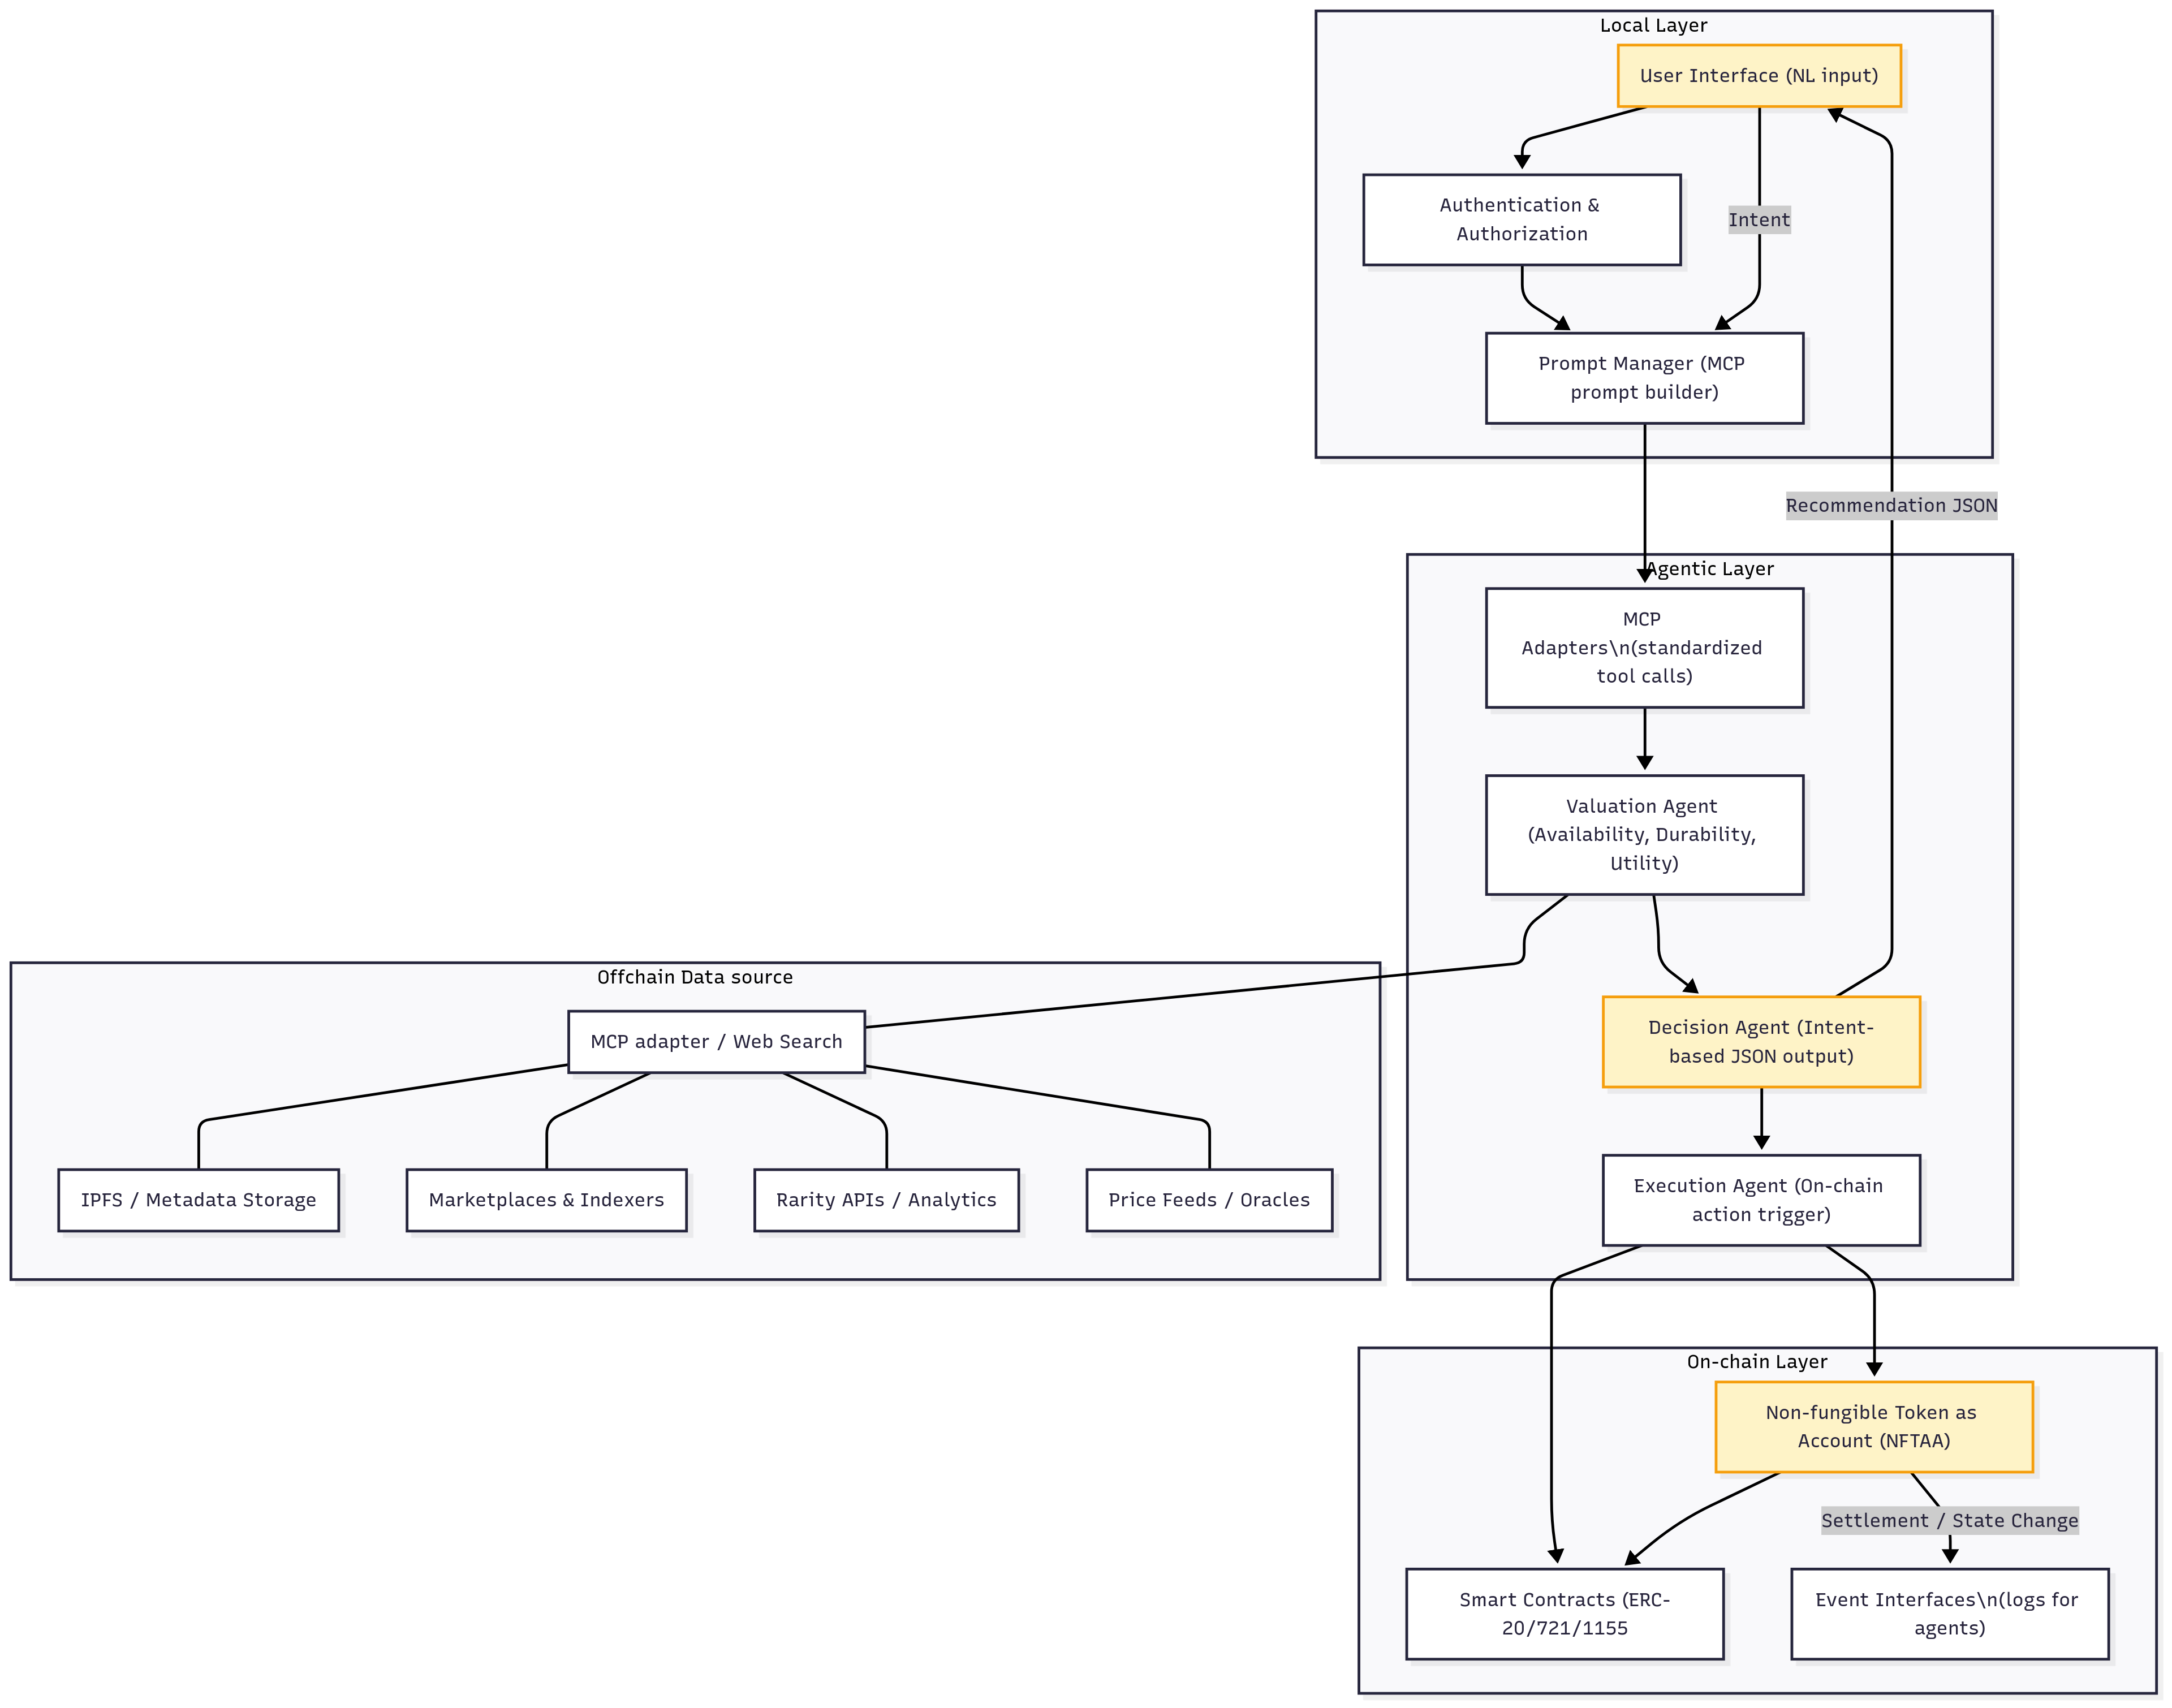
\includegraphics[width=\columnwidth]{images/architecture.png}
    \caption{Architecture of the agentic system}
    \label{fig:architecture}
\end{figure}

In the Figure \ref{fig:architecture} we can see the proposed architecture for agentic systems in the context of Internet of Value. System is composed from four parts: Data layer, Agentic layer and Local layer and Onchain layer.  At the bottom, the on-chain layer anchors the system through smart contracts that implement token standards, access control, and event emission. These contracts act as an interface for agentic system, ensuring that every transaction is transparent and verifiable.
Agentic layer is a semi-autonomous layer of AI agents that is able exectute onchain smart contracts and communticate with the user. Within this layer, valuation agents collect information about assets from distributed sources such as IPFS, marketplaces, rarity tools, and price feeds. Decision agents transform these findings into structured recommendations that are adjusted according to user intent, while execution agents carry out the approved actions by interacting directly with the blockchain. The agentic layer communicates with external data sources through Model Context Protocol adapters, guaranteeing predictable and reproducible tool invocation.Finally, the local layer forms the entry point for human participants. Here, intent is expressed in natural language, authenticated, and transformed into standardized prompts before entering the agentic layer. By structuring the system in this way, the architecture closes the loop between human intention, autonomous reasoning, and decentralized settlement, while maintaining security, transparency, and extensibility.

The addition of the data layer emphasizes that any meaningful valuation of digital assets must be grounded in reliable information streams. This layer aggregates and normalizes data from heterogeneous sources, including decentralized storage systems such as IPFS, public block explorers, centralized and decentralized marketplaces, rarity ranking services, and external price feeds oracles. The primary role of the data layer is to provide structured, machine-readable input to the agentic layer, abstracting away differences between providers while preserving verifiability of origin. In this sense, the data layer functions as the knowledge substrate upon which agents perform their contextual analysis.

The interaction between these four layers follows a continuous cycle. The process begins in the local layer, where a user formulates their intent. This intent is authenticated, logged, and transformed into a standardized prompt. The agentic layer receives this prompt and coordinates the work of specialized agents. Valuation agents query the data layer to retrieve asset-specific information, assessing availability, durability, and utility. Decision agents then combine these assessments with the user’s expressed intent to compute a context-dependent value function and produce a structured recommendation. If the recommendation is approved by the user, execution agents translate it into concrete blockchain transactions, which are carried out within the on-chain layer. Smart contracts enforce access control, update state, and emit events, which in turn can be captured by the data layer to close the information loop.

By organizing the architecture in this manner, we achieve a modular yet tightly coupled system. Each layer maintains a well-defined responsibility: the local layer mediates human interaction, the data layer provides trustworthy information, the agentic layer enables cognition and decision-making, and the on-chain layer guarantees settlement and immutability. This separation of concerns not only increases the robustness of the overall design but also ensures extensibility. New data providers, agent types, or smart contract modules can be integrated without disrupting the integrity of the system. Moreover, the reliance on open token standards and decentralized storage solutions ensures interoperability across different EVM-based and non-EVM chains, while the use of MCP secures predictable behavior of autonomous agents. Together, these properties create an architecture that is transparent, secure, and adaptable—qualities that are essential for advancing the Internet of Value through agentic systems.


\subsection{Agentic Layer}

Without any doubt, the agentic layer is a core component of our architecture. It mediates between human intent, raw blockchain data, and the on-chain settlement layer, enabling intelligent and context-aware interactions with digital assets. Unlike the on-chain layer, which is by nature deterministic and immutabile, the agentic layer introduces flexibility, reasoning, and adaptation through the use of autonomous AI processes. Its components work in a coordinated manner: valuation agents transform heterogeneous data into structured metrics, decision agents contextualize these metrics according to user intent, execution agents operationalize validated decisions on-chain, and MCP adapters ensure that communication with external tools remains predictable and reproducible. Together, these components create a closed loop that begins with user intent and culminates in verifiable blockchain state changes, thereby embedding cognition into the Internet of Value.

\begin{figure}[!h]
    \centering
    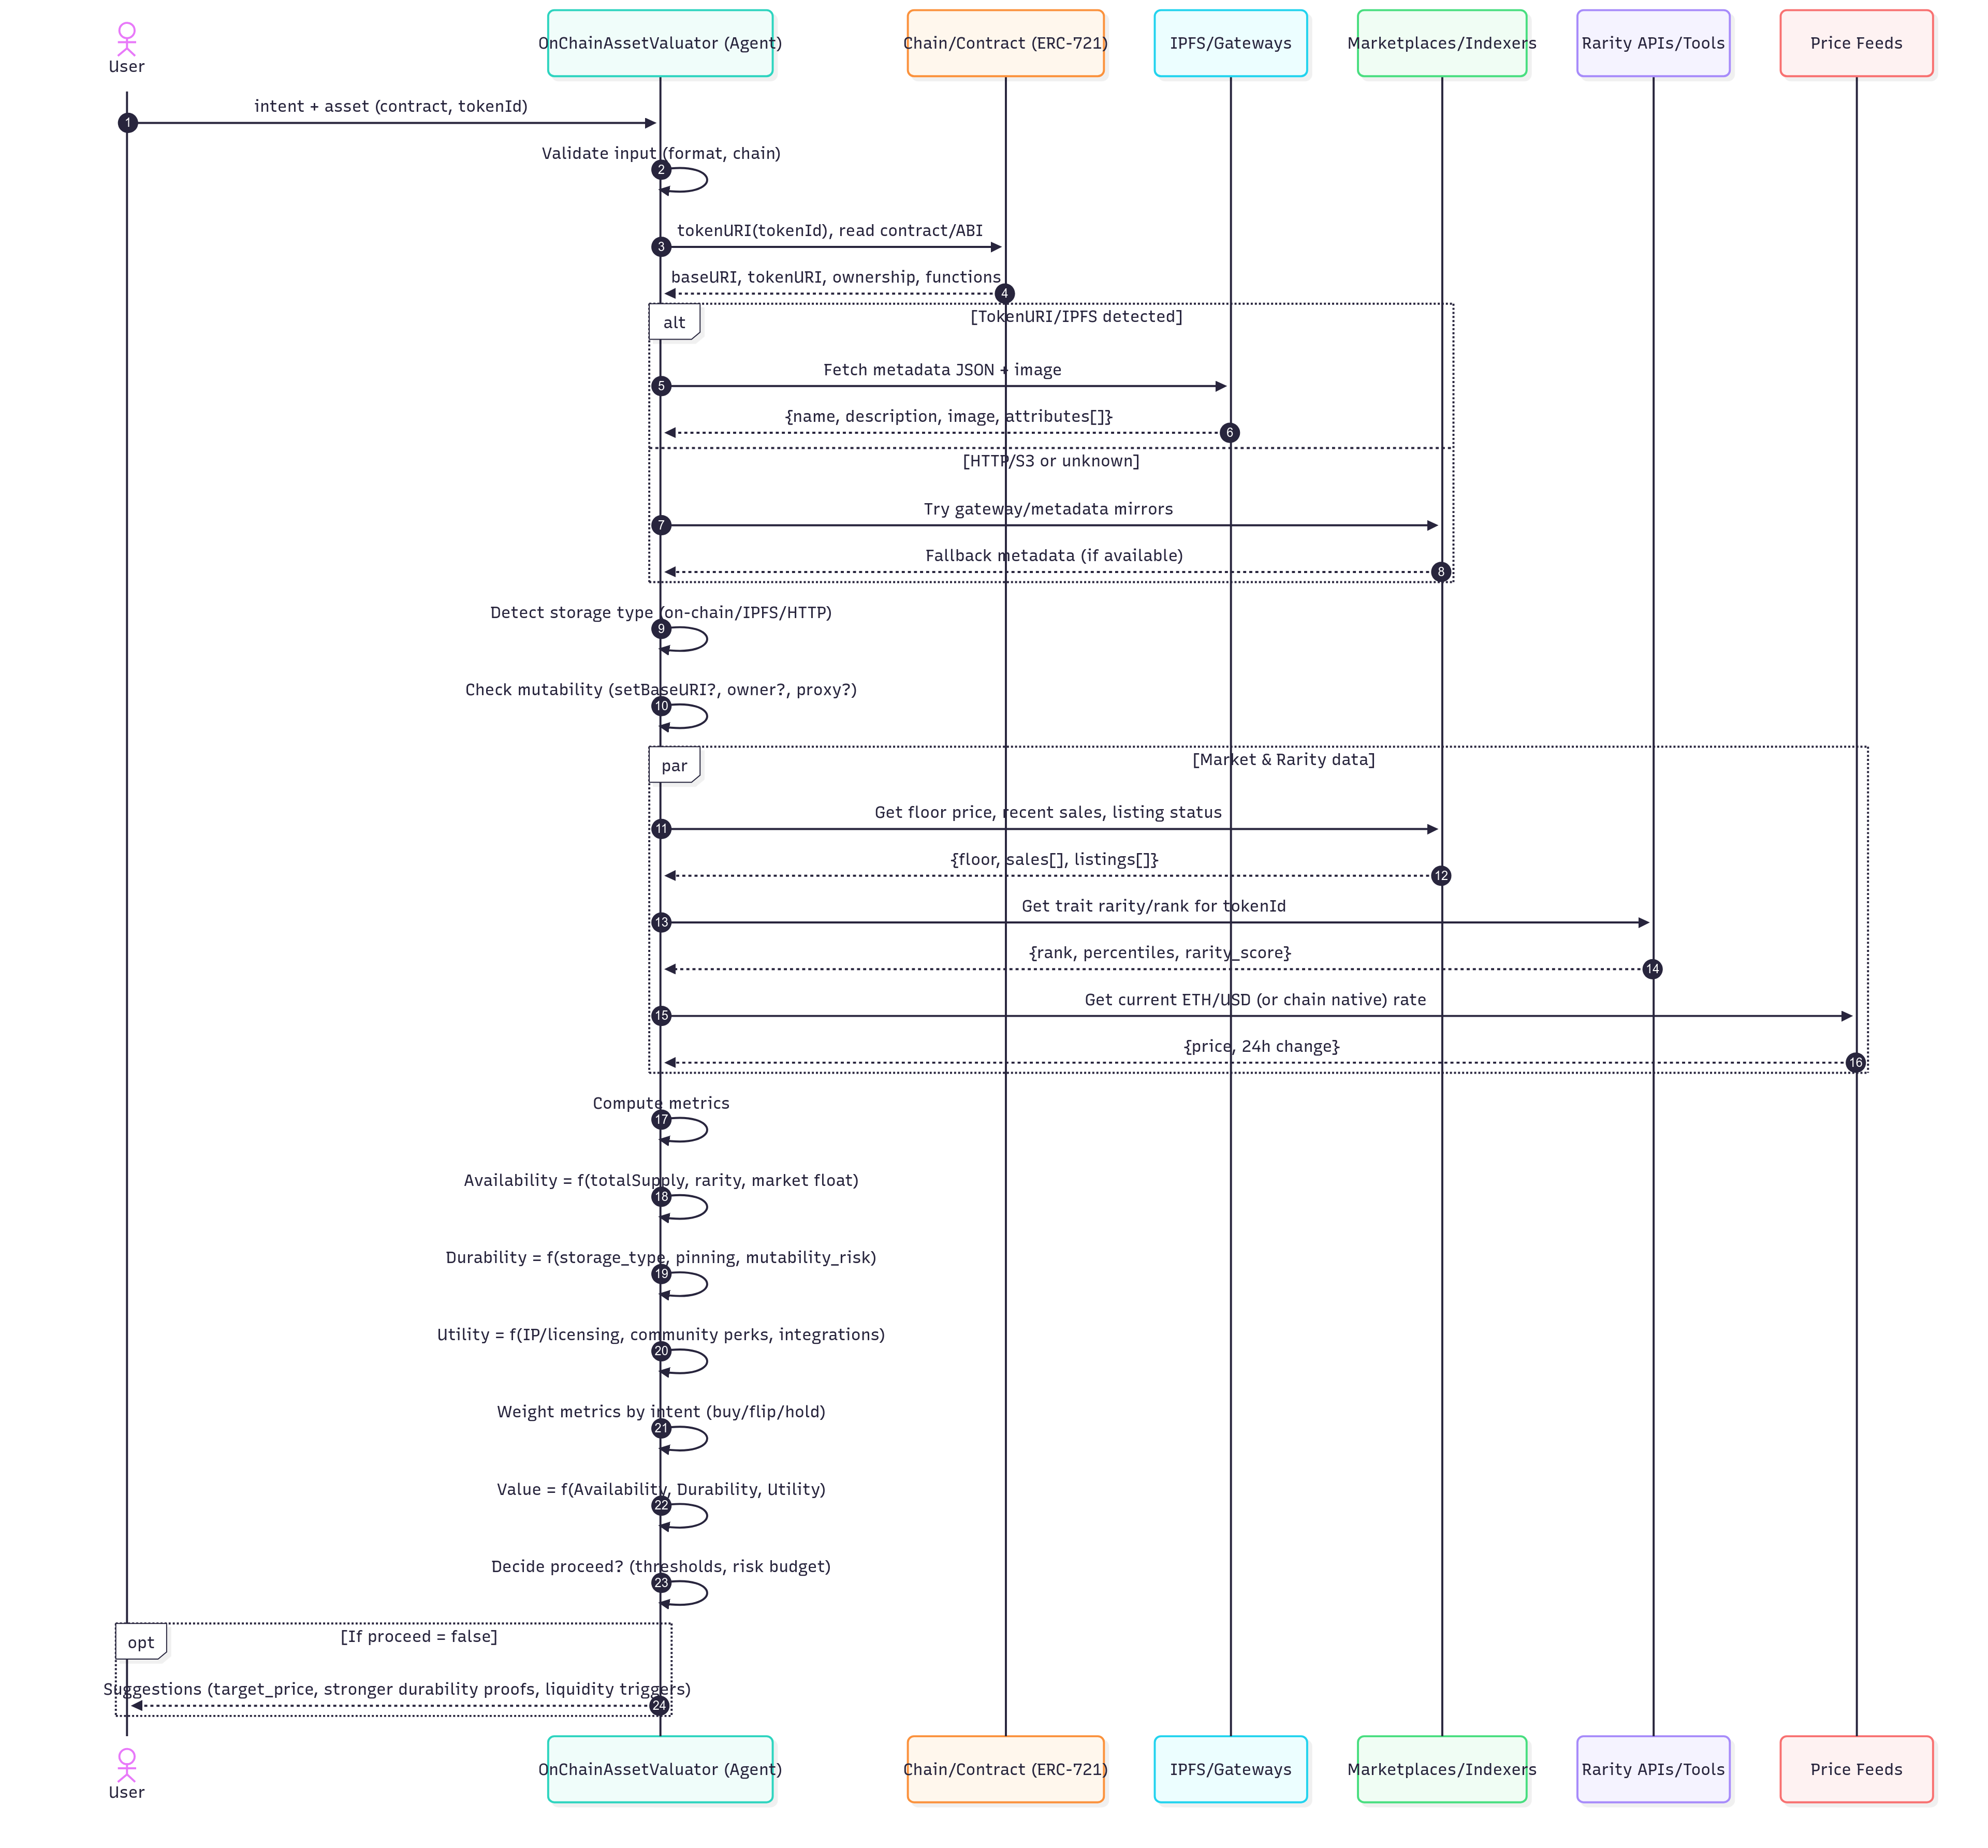
\includegraphics[width=\columnwidth]{images/agentic-sequence.png}
    \caption{Flow from user to Valuation Agent}
    \label{fig:agentic-sequence}
\end{figure}

The valuation agent is responsible for the contextual analysis of assets within the Internet of Value. Its primary task as shown in the Figure \ref{fig:agentic-sequence} is to compute the three dimensions of value: availability, durability, and utility. To achieve this, the agent continuously acquires data from heterogeneous sources such as blockchain explorers, decentralized storage networks (e.g., IPFS), marketplaces, rarity analytics platforms, and oracle services. The agent normalizes this information into a consistent internal representation, which allows it to compare diverse assets across collections and chains. In the context of NFTs, the valuation agent determines scarcity by inspecting the overall token supply and trait distribution, evaluates durability by examining metadata storage and contract mutability, and assesses utility by identifying existing and potential use cases such as licensing opportunities or access rights. Its output is a structured profile of the asset that feeds directly into higher-level reasoning tasks. The valuation agent thus acts as the analytical core of the system, translating raw data into interpretable metrics that can later be weighted according to user intent.



How can large-language model can become expert in asset valorization? That's an important question. It starts with a system prompt, that can be imagined as a set of permament instructions of how AI model should behave. In Listing \ref{lst:systemprompt} we can see a excerpt from system prompt for valuation agent.

\begin{lstlisting}[caption={Executing hook from}, label={lst:systemprompt}]
You are **OnChainAssetValuator**, a specialized AI agent that analyzes, values, and advises on blockchain / NFT / token assets.
Your purpose is: **asset identifier (contract + token ID or project name)**, you will:

1. Fetch on-chain & off-chain data (metadata storage, contract mutability, trait rarity, price history, utility roadmap).
2. Compute three core metrics for the asset: **Availability (scarcity)**, **Durability (resilience of metadata, mutability risk)**, **Utility (present & prospective usefulness / monetization)**.
4. Output a Markdown object with at least the following fields:
   - `Availability` description
   - `Durability` description
   - `Utility` description
   - `Overall sumarry`
   - `Reasoning`

Behavioral constraints & guidelines:
- Always validate that metadata conforms to standards (ERC-721 metadata, OpenSea schema).
- Identify whether metadata is on-chain, IPFS, centralized, or hybrid; check for mutability (e.g. `setBaseURI`, upgradeable logic).
- Use real market data (floor price, recent sales) and rarity data where available.
- Add valuation logic for possible **intents**: e.g. for buying, favor lower risk and safer durability; for flipping weight momentum and liquidity.
- Avoid hallucinating data; if a metric is unavailable, state unknown rather than guessing.
- Suggest conditions under which the asset could become more valuable(e.g. lower price, proof of immutable metadata, stronger utility roadmap).
- Always output strictly valid Markdown.

From this point, I (the user) will simply provide you with **intent + asset identifier**, e.g.:

> asset: 0xbd3531da5cf5857e7cfaa92426877b022e612cf8 / 1419
or
> asset: https://opensea.io/item/ethereum/0xbd3531da5cf5857e7cfaa92426877b022e612cf8/1419

You should then produce the markdown valuation and recommendation accordingly.
\end{lstlisting}

Once we have output we can pass the output to decisiion agent. However thanks to our modular architecure we can plug and play any amount of models in the pipeline.

\subsubsection{Decision Agent}

The decision agent transforms analytical insights into actionable recommendations. While the valuation agent provides a factual description of an asset’s characteristics, the decision agent incorporates user intent into the reasoning process. Intent may range from speculative investment and long-term holding to immediate consumption or resale. As Listing \ref{lst:structuredoutput} shows we use as structured JSON output to represent the analysis of the decision agent. By applying a weighted function that combines availability, durability, and utility with the contextualized intent, the decision agent generates a quantitative value score. This score is accompanied by qualitative reasoning and a confidence measure, ensuring that outputs are interpretable and auditable. The decision agent also considers edge cases, such as incomplete data or high volatility, and adjusts its confidence accordingly.
% Importantly, the agent outputs its recommendation in structured formats such as JSON, which guarantees compatibility with downstream tools and ensures reproducibility: the same input prompt consistently produces the same structured response. In this way, the decision agent represents the cognitive bridge between objective evaluation and subjective decision-making.

\begin{lstlisting}[caption={Structured output format of decision agent}, label={lst:structuredoutput}]
{
  "confidence": "Model confidence in the recommendation.",
  "value": {
    "score": "Overall value score on the given scale.",
    "scale": "Scale used for scores.",
    "weights": {
      "availability": "Weight for Availability component.",
      "durability": "Weight for Durability component .",
      "utility": "Weight for Utility component."
    },
    "components": {
      "availability": {
        "score": "Component score on the specified scale.",
        "note": "Short justification for the component score."
      },
      "durability": {
        "score": "Component score on the specified scale.",
        "note": "Short justification for the component score."
      },
      "utility": {
        "score": "Component score on the specified scale.",
        "note": "Short justification for the component score."
      }
    }
  },
  "proceed": "Whether the user should proceed with the stated intent.",
  "reasoning": "Brief rationale explaining the decision."
}
\end{lstlisting}


The execution agent is responsible for operationalizing the recommendations produced by the decision agent. Once an action is validated by human-in-the loop process, such as purchasing an NFT, transferring a token, or interacting with a governance contract, the execution agent securely interfaces with the blockchain. Since agent knows parameters of the inspected data such as smart contract address, address of the account or token id, we are able to submit valid on-chain transaction along with its simulation. The execution agent manages cryptographic signing, nonce management, and gas optimization, thereby shielding the user from low-level technical complexities. It also monitors the blockchain for confirmations and provides verifiable proofs of execution back to the user, such as transaction hash. To enhance resilience, the execution agent is designed with rollback and fail-safe strategies: in cases where execution fails, it can revert the action or notify the user of the cause. The transparency of its actions is guaranteed by on-chain settlement, which produces immutable records of every decision.]


% talk about liquspell

However, the main question remains unanswered. How does system understands from simple english propmpt that it should execute on chain transaction? Luckily modern LLMs can be extended with tools, can expand capabilities of the model. In the Listing \ref{lst:tooldefiniton} we see a definition of the tool that can teleport DOT from one parachain to another parachain with givven amount. These tools are instantly available in the context of the LLM and need to be defined by the time we initialize connection with the agent.
However, what if we need ability to control external services when needed to respond to a user's prompt? That's the reason why we need  Model Context Protocol.
MCP adapters provide the standardization and interoperability necessary for reliable agent-tool interactions. They serve as the middleware that translates natural language prompts and structured agent requests into deterministic tool calls. Without this abstraction, the behavior of large language models may become unpredictable, as the same prompt could trigger different tool invocations across sessions. MCP adapters enforce consistency by binding prompts to fixed function signatures, ensuring that identical inputs always yield the same outputs. Within the agentic layer, MCP adapters connect valuation agents to data sources, decision agents to external evaluators, and execution agents to blockchain interfaces. They also support extensibility: new tools can be registered without modifying the core agent logic, enabling the architecture to evolve alongside technological advances. By incorporating MCP, the system maintains predictability, reproducibility, and auditability—qualities that are essential for a framework that aspires to operate within the Internet of Value.



\begin{lstlisting}[caption={Tool definition for OpenAI GPT-4o model}, label={lst:tooldefiniton}]
export const teleportTokenTool: ToolConfig < TeleportTokenArgs > = {
  definition: {
    type: 'function',
    function: {
      name: 'teleport_tokens',
      description: 'Teleport tokens from one chain to another with defined currency',
      parameters: {
        type: 'object',
        properties: {
          from: {
            type: 'string',
            description: 'The name of the source chain'
          },
          to: {
            type: 'string',
            description: 'The name of the destination chain'
          },
          symbol: {
            type: 'string',
            description: 'The symbol of the token on the source chain, if no symbol is provided, assume it is DOT'
          },
          amount: {
            type: 'string',
            description: 'The amount of tokens to swap, multiply the amount by 1e10'
          },
          receiver: {
            type: 'string',
            description: 'The receiver of the tokens, must be valid in AccountID32 or AccountKey20 format '
          },
        },
        required: ['from', 'to', 'receiver', 'amount']
      }
    }
  }
}
\end{lstlisting}

However, one of the unique features of our architecture is the transcation entrypoint that will be discussed in the next sub section.

\subsection{On-chain Layer}

The on-chain layer constitutes the settlement and trust foundation of the proposed architecture. It is here that all agentic decisions are ultimately anchored and enforced through blockchain primitives. Unlike the agentic layer, which is adaptive and reasoning-oriented, the on-chain layer provides determinism, immutability, and verifiability, ensuring that every executed action is transparently recorded in the distributed ledger.

At the core of this layer lies the \textbf{Non-fungible Token as Account (NFTAA)} concept, as introduced by Valastin et al.~\cite{valastin2024nftaa}. NFTAA extends the traditional ERC-721 model by representing each non-fungible token not only as a unique asset but also as an autonomous account with programmable logic. In this model, NFTs become active participants in the blockchain ecosystem: they can hold balances, execute transactions, and interact with other smart contracts directly. This abstraction is particularly powerful in the context of the Internet of Value, as it allows NFTs to serve simultaneously as identity containers, value carriers, and execution agents. By embedding account functionality within NFTs, the architecture gains a higher degree of composability and interoperability across decentralized applications.

One of the advantages of NFTAA is ability to operate and own standard fungible and non-fungible asset, therefore we allow assets to be exchanged, fractionalized, or collateralized using widely adopted token standards. In addition, smart contracts define access control rules and enforce invariants, guaranteeing that only authorized execution agents may trigger sensitive state transitions. Compared to existing solution such as Virtuals that is using ERC-6551, with NFTAA we are allowed do design custom design custom semantics and override default constraints that are present in 6551 such as registry-based approach.

Third state of the art solution that we researched is event-based actions for AI agent. In short term smart contracts can emit events that can be processed by the external services. While reading live events from chain, we can spawn AI agent to react to this on-chain action. This creates so called blokchain-in-the-loop system.
 instead of having user that approves or denies actions, blockchain can trigger various action available on the agent. Therefore Event logs provide the bridge between deterministic blockchain state and the agentic layer’s reasoning processes, as blockchain can trigger various action on agents or agents are able to maintain an up-to-date context of particular asset. This design ensures that the agentic system remains reactive to blockchain dynamics without compromising security or transparency.


\subsection{Local Layer}

The local layer functions as the human–agent interface of the architecture, ensuring that end users can express intent, maintain oversight, and retain sovereignty over actions performed within the system. While the agentic and on-chain layers handle cognition and settlement, the local layer emphasizes usability, accountability, and security. It is composed of three primary components: the user interface, authentication and authorization mechanisms, and the prompt manager.

The user interface provides the entry point for human participants into the Internet of Value. Its role is to abstract the technical complexities of blockchain interactions and agentic reasoning, enabling users to communicate their intent in natural language or simplified structured form. Instead of requiring knowledge of token standards, contract addresses, or transaction parameters, the user can issue a straightforward request such as ``evaluate the value of NFT \#1419'' or ``buy this token if it falls below ten ether.'' The interface translates such expressions into a formalized representation that can be consumed by downstream processes. By lowering the barrier to entry, the interface widens participation in decentralized economies, supporting inclusivity while reducing the risk of errors that could occur in manual transaction crafting. Furthermore, the interface provides visual feedback in the form of structured recommendations, confidence scores, and audit trails, ensuring that the user remains informed about the system’s reasoning and actions.


Given the sensitivity of executing blockchain transactions, robust mechanisms for authentication and authorization are critical in the local layer. Authentication ensures that only legitimate users can access the system, typically by leveraging cryptographic wallets, decentralized identity frameworks, or multi-factor authentication schemes. Authorization extends this protection by defining which actions a particular user is permitted to perform. For instance, a user may be allowed to request asset valuations but not to execute token transfers unless additional verification is provided. This separation of authentication and authorization aligns with principles of least privilege, minimizing attack surfaces while preserving usability. The design also supports non-repudiation, as all authenticated actions can be cryptographically attributed to the initiating user, which is vital for accountability in a decentralized context.

The prompt manager is responsible for transforming human intent into deterministic machine-readable instructions. This component plays a crucial role in bridging the gap between natural language input and predictable agent behavior. It takes the user’s request, validates it against the system’s schema, and compiles it into a prompt that conforms to the Model Context Protocol (MCP). This ensures that when the same prompt is provided to the agentic layer, it always produces the same sequence of tool invocations and responses. The prompt manager also embeds contextual metadata, such as user intent, prior interaction history, and execution constraints, into the generated prompt. By maintaining an audit log of all prompts and their corresponding outputs, it supports reproducibility and accountability, allowing external reviewers to verify that actions were executed faithfully. In addition, the prompt manager enforces safeguards by rejecting malformed or unauthorized requests, preventing the agentic layer from being manipulated into unsafe or unintended behaviors.


Additionally, using blockchain-the-loop mechanism local layer acts as entry point for agents to react to the blockchain events.

\subsection{Usage of Agents in on-chain governance}

In traditional blockchain-based governance systems, human actors (token holders, delegates, DAO committees) propose, vote, and execute governance decisions. These processes rely heavily on manual intervention, periodic coordination, and human diligence. As governance complexity increases (across multi-chain protocols, cross-project dependencies, frequent parameter upgrades), this manual model becomes a bottleneck. Agentic systems, when integrated into the governance plane, promise to automate, optimize, and scale governance in a trust-minimized and auditable way.

In this section we will expand on real world use case of using our state of the art architecure for exchanging assets amoung entities in the Internet of Value, with main focus on Polkadot.
At the point of writing Polkadot treasury holds more 10.8 Milion of DOT\footnote{Around ~43 Milion of USD}. That could be distributed, towards people. However many people claim that pricing of the proposal is unjusted therefore outflow of funds and its overall value seems to be mispriced.
An agentic system could be used to evaluate the proposals based on the contextual asset value framework. Therefore each proposal would be evaluated based on its availability, durability and utility. The decision agent would then analyze the data and make a recommendation on whether to approve or reject the proposal. The execution agent would then execute the decision on-chain.

How does it work in practice? Let's say that a new proposal is submitted to the Polkadot treasury. Using blockchain-in-the-loop approach, agent is spawned up by the Submitted event on the Referenda pallet\footnote{https://polkadot.subscan.io/event?module=referenda&event_id=Submitted}. The valuation agent would then collect data about the proposal, such as its budget, timeline, and expected outcomes. The decision agent would then analyze the data and make a recommendation on whether to approve or reject the proposal. By the approval from human would then execute the decision on-chain.

This approach has several benefits. Firstly, it would ensure that proposals are evaluated based on objective criteria, rather than subjective opinions. Secondly, it would reduce the workload on human actors, allowing them to focus on more strategic tasks. Finally, it would increase the transparency and accountability of the governance process, as the final decision is recorded on-chain.

This use case illustrates how agentic systems can enhance blockchain governance by automating decision-making processes while maintaining trust and transparency. By leveraging the strengths of both human judgment and autonomous reasoning, such systems can help decentralized communities manage resources more effectively in an increasingly complex ecosystem.

This creates a strong loop between human intent, autonomous reasoning, and decentralized settlement, enabling more efficient and scalable governance in the Internet of Value.

However, there are still many open questions and challenges that need to be addressed. For example, how to ensure that the agents are aligned with the values and goals of the community? How to prevent manipulation or gaming of the system? How to balance automation with human oversight? These are valid questions, thus we will explain them in the following paragraphs.
As we have learned so far, the decision agent produces structured output that includes confidence score and reasoning. This allows human actors to review the agent's recommendations and make informed decisions. Additionally, agent can take similar proposes from the past and take them into consideration when making recommendations. This historical context can help the agent to avoid repeating mistakes and to learn from past successes. Additionall context can be added via local layer where human can provide additional context about the proposal such as W3F voting recommendation\footnote{https://medium.com/web3foundation/w3f-opengov-proposal-voting-guidelines-543ff7faba03}.



% \subsection{Advancing Beyond the State of the Art} \label{sec:advancing-sota}

% Existing systems demonstrate compelling directions—Virtuals excels at tokenized agent identity and community ownership, Autonolas at fault-tolerant multi-agent services and cross-chain operation, and Griffain at natural-language usability on a high-throughput chain. Yet, across these approaches we observe four persistent gaps that limit reliability and credible autonomy in the Internet of Value: (i) weak reproducibility of agent decisions, (ii) incomplete verifiability of off-chain cognition, (iii) coarse-grained authority delegation, and (iv) fragile links between NFT metadata durability and on-chain execution policy. Our architecture addresses these deficits through a set of design principles and mechanisms that jointly improve predictability, trust, and safety without sacrificing usability.

% First, we introduce \emph{deterministic, reproducible cognition} for agent decisions. Rather than treating LLM reasoning as an opaque black box that returns an action, the agentic layer implements an MCP-governed ``\textbf{Plan--Act--Verify}'' loop with explicit artifacts: a normalized intent specification, a structured tool plan, and a signed action proposal. Each artifact is hashed (content-addressed) and bound to its inputs (prompt, tools, versions, chain state snapshots). The resulting \emph{decision provenance tuple}—\texttt{\{prompt\_hash, toolset\_digest, model\_digest, data\_fingerprints\}}—is committed on-chain prior to execution. By committing these hashes to a settlement contract, any observer can later reconstruct the decision path and check that identical inputs would lead to identical actions. This creates a reproducible pipeline missing from Virtuals and Griffain, and more explicit than Autonolas’ developer-oriented registries.

% Second, we make \emph{off-chain cognition verifiable} at useful granularity. Full cryptographic proofs of LLM inference remain costly; instead, we combine (a) \emph{input/data attestations} from the data layer (Merkleized snapshots of IPFS CID lists, marketplace responses, and price feed reads), with (b) \emph{policy-constrained simulation} on-chain. Before a state-changing transaction is broadcast, the execution agent must submit a \textit{preflight} that references the decision provenance tuple and passes a set of on-chain predicates: price slippage bounds, maximum spend caps, trait/rarity thresholds, oracles’ staleness limits, and metadata immutability constraints. These predicates are expressed in a compact DSL compiled to EVM checks. The chain thus verifies that the proposed action is consistent with the agent’s declared policy and the attested inputs. Compared to Virtuals’ token governance and Griffain’s delegated wallets, this creates a stronger guarantee that the chain enforces what the agent claimed to reason about.

% Third, we replace coarse delegation with \emph{capability-based authority} using account abstraction. Concretely, users delegate a \emph{capability NFT} (ERC-721) or \emph{session key} (ERC-4337/EIP-7702 style) to the execution agent. The capability encodes fine-grained constraints: spend ceilings, allowed protocols, token allowlists, signature lifetimes, and rate limits. Capabilities are revocable and upgradable under multisig or time-lock; the execution contract validates them via ERC-1271. This is safer than Griffain’s single delegated key and more user-centric than Virtuals’ agent-token governance, while remaining simpler to adopt than Autonolas’ full multi-operator stacks for many consumer use cases.

% Fourth, we bind \emph{NFT durability} directly into agent policy and settlement. The on-chain layer maintains a \emph{Value Registry} that stores machine-verifiable attestations for Availability, Durability, and Utility. Durability is not a narrative tag but a cryptographic condition: the registry records the tokenURI base, IPFS CIDs for metadata/images, optional freeze proofs (e.g., absence of \texttt{setBaseURI}, renounced ownership, or governance constraints), and pinning attestations. Agent policies can require that ``Durability $\geq$ threshold'' (e.g., IPFS-only, immutable base URI, staleness under $x$ days) before allowing a purchase or collateralization. This closes the gap where current systems evaluate NFTs but do not \emph{enforce} durability in execution flows.

% These innovations are complemented by pragmatic safety and market mechanisms. Transactions are routed through private mempools or protected relays to reduce MEV exposure; every order includes deterministic slippage and deadline guards generated from the Plan step. Where multi-agent reliability is required, we adopt a \emph{lightweight quorum} scheme: independent agents run identical MCP pipelines, sign EIP-712 action proposals, and threshold-approve the execution; this borrows Autonolas’ spirit of redundancy without imposing its operational complexity on simpler tasks. To prevent silent regressions, all models, tools, and prompts are \emph{versioned} and pinned; any change produces a new toolset digest and therefore a distinct provenance tuple, surfacing drift as an explicit review event rather than an invisible risk.

% Our approach also improves developer and user ergonomics. For developers, MCP adapters expose a minimal, typed surface that transforms heterogeneous data (IPFS, explorers, DEX/market APIs, rarity analytics) into a canonical schema with cryptographic fingerprints. For users, the local layer offers intent templates that compile into policies and capabilities automatically; humans specify \emph{what} they want, while the system derives \emph{how} to do it safely. In contrast to Virtuals’ governance-driven feature evolution and Griffain’s natural-language immediacy, our system preserves the same ease of use but attaches verifiable guardrails and reproducibility by default.

% Finally, we define a rigorous evaluation protocol to substantiate superiority over SOTA. We measure (i) decision reproducibility (identical-input same-output rate), (ii) action validity (on-chain predicate pass rate), (iii) safety incidents (MEV losses, out-of-policy executions), (iv) time-to-settlement and gas overheads for preflight and capability checks, and (v) user-acceptable latency and satisfaction in A/B tests. We further report \emph{durability enforcement efficacy} by auditing how many candidate NFTs are filtered by policy and the realized impact on post-purchase metadata availability. These metrics translate thesis claims—predictability, verifiability, and safety—into empirical evidence, enabling a fair comparison against Virtuals, Autonolas, and Griffain within the IoV context.

% In summary, the proposed architecture \emph{outperforms current SOTA} by making agent cognition reproducible, off-chain reasoning verifiable, delegation granular and revocable, and NFT durability enforceable at execution time—all while preserving the usability advances that have driven adoption of existing systems. This combination advances the Internet of Value toward trustworthy, intent-driven autonomy.
